%----------------------------------------------------------------------------------
% Exemplo do uso da classe tcc.cls. Veja o arquivo .cls
% para mais detalhes e instruções.
%----------------------------------------------------------------------------------
\chapter{\label{chap:intro}Introdução}

%%%%%%%%% TEM QUE ESTAR EM ORDEM ALFABETICA %%%%%%%%%%

%\sigla{CC}{Cloud Computing}

\sigla{BGP}{Border Gateway Protocol}
\sigla{CoAP}{Constrained Application Protocol}
\sigla{DTLS}{Datagram Transport Layer Security}
\sigla{HTTP}{Hypertext Transfer Protocol}
\sigla{IP}{Internet Protocol}
\sigla{LE}{Low Energy}
\sigla{NIST}{National Institute of Standards and Technology}
\sigla{REST}{Representational State Transfer}
\sigla{SDK}{Software Development Kit}
\sigla{TCC}{Trabalho de Conclusão de Curso}
\sigla{TCP}{Transmission Control Protocol}
\sigla{RFC}{Request for Comments}
\sigla{UDP}{User Datagram Protocol}

% Comando para inserir abreviaturas.
%
% \abrev{Abrev}{Abreviatura}
% \abrev{Inform}{Informática}
%
% Comando para inserir símbolos. Estes irão aparecer em ordem
% de ocorrência, já que o número da página está presente na lista
% de símbolos.
% \simbolo{Hz}{Hertz}
% \simbolo{$\pi$}{Constante com valor aproximado de $3.1415926$}%
%
% bom site sobre BRTs
% http://www.brtdata.org/location/latin_america/mexico/mexico_city
%

\section{Contextualização}

A computação em nuvem tem sido amplamente adotada nos últimos anos por usuários finais e empresas de vários segmentos e portes.
As facilidades proporcionadas por este modelo de computação faz com que exista tal preferência, pois, segundo a definição adotada
pelo NIST \cite{Mell:2011}, computação em nuvem é um modelo que permite acesso a um conjunto compartilhado de recursos computacionais configuráveis que podem ser provisionados e liberados  com um pequeno esforço de gerenciamento ou interação com provedor de acesso.
Toda essa flexibilidade pode justificar o aumento no emprego desse modelo de computação.

Como a computação em nuvem não é panacéia\footnote{Mecanismos ou práticas que, hipoteticamente, são capazes de solucionar os problemas e/ou dificuldades \cite{definition:panaceia}.}, podemos utilizar a definição de Bonomi, Milito, Zhu e Addepalli \cite{Bonomi:2012} que relata que a computação em nuvem libera as empresas e os usuários finais de muitos detalhes de especificações.
Essa facilidade torna-se um problema para aplicações sensíveis à latência, que requerem que nós próximos atendam suas necessidades de forma eficiente. 
Como a interação entre os nós e os servidores na nuvem ocorrem através da internet, a baixa latência torna-se indispensável para aplicações que requerem eficiência na comunicação entre nós (por exemplo robôs, drones, e carros autônomos).
Portanto, há uma lacuna entre aplicações que já utilizam modelos de computação em nuvem e aplicações que necessitam de baixa latência de rede e comunicação entre nós próximos, e é nesse hiato que a computação em névoa surge.

A computação em névoa é um assunto relativamente novo e teve sua primeira definição, dada pela Cisco Systems\footnote{Empresa estadunidense líder na fabricação de equipamenteos de rede \cite{ciscoSystems}.} em 2012, como uma extensão do paradigma de computação em nuvem que provê armazenamento, computação e serviços de rede entre dispositivos finais e os servidores na nuvem \cite{DBLP:journals/corr/RomanLM16}. 

Atualmente a computação em névoa tornou-se um paradigma próprio e não mais uma mera extensão da computação em nuvem, e desse
paradigma criou-se o conceito de \textit{fog nodes}, que abrangem desde dispositivos finais com baixa capacidade computacional até servidores poderosos na nuvem.
Assim, os \textit{fog nodes} passam a fazer parte da implementação dos serviços em nuvem.
O que torna a computação em névoa interessante é a capacidade dessa variedade de dispositivos cooperarem uns com os outros de forma distribuída.

\begin{figure}[htb!]
    \centering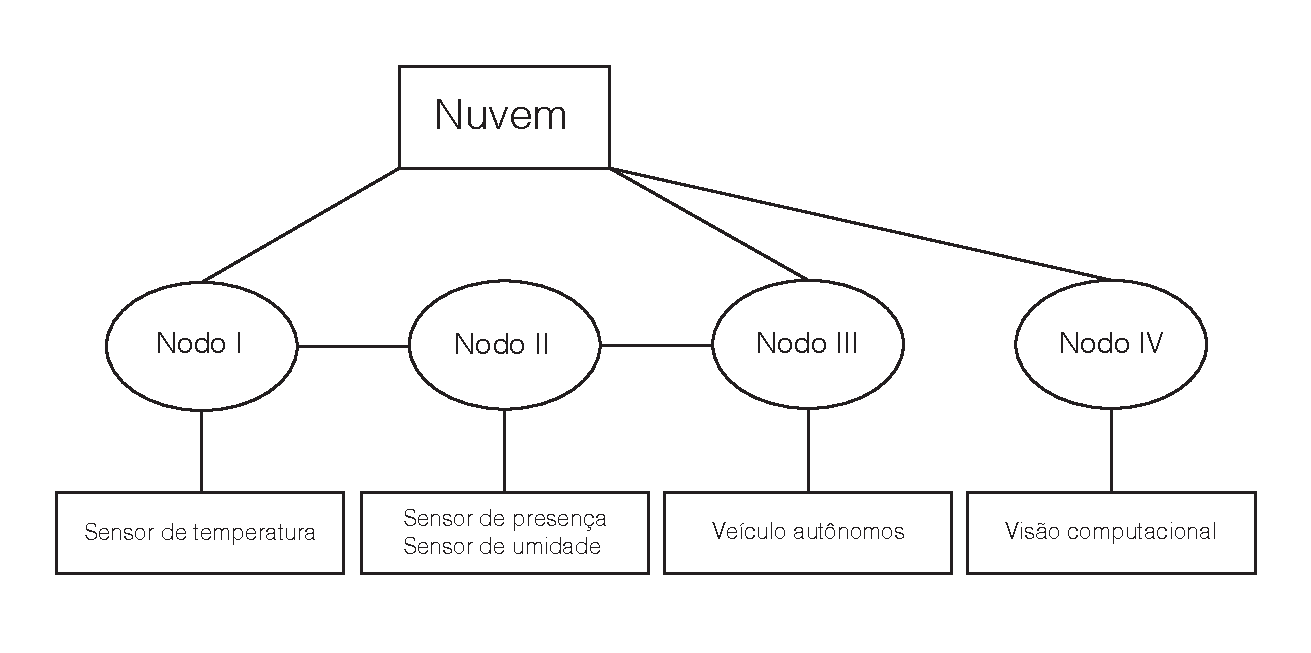
\includegraphics[width=.5\textwidth]{fig1.pdf}
    \caption
    {\label{fig:fig1} Organização arquitetural.} \cite{archfog:2017}
\end{figure}

Em uma abordagem \textit{bottom-up}, podemos descrever a arquiterura da computação em névoa como um conjunto de \textit{edge devices}\footnote{Dispositivo que controla o fluxo de dados no limite entre duas redes \cite{edgeDevices}.} que se comunicam com os \textit{fog nodes}, e esses com servidores centrais.
Entretanto, a comunicação entre os \textit{fog nodes} e os servidores centrais nao é essencial para a execução dos serviços em névoa \cite{DBLP:journals/corr/RomanLM16}.
A Figura \cite{archfog:2017} representa este conceito de computação em névoa.

\section{Motivação e justificativa}

De acordo com Vaquero e Rodero-Merino \cite{Vaquero:2014}, serão sete os desafios que a computação em névoa deverá enfrentar para se tornar realidade.
Os problemas referentes à padronização, descoberta e sincronização são os motivadores deste trabalho, uma vez que atualmente não existem mecanismos
no qual um membro da rede, seja ele um dispositivo com limitações de memória e processamento ou um computador, mapeiem os recursos disponíveis e divulgue os seus na rede.

A ausência desses mecanismos faz com que cada membro interaja exclusivamente com seus recursos, portanto, não há compartilhamento entre os nodos da rede.
O motivo pelo qual os nodos não consomem os recursos de seus vizinhos está no desconhecimento da existência dos mesmos, sendo assim, é inviável utilização de um recurso que não esteja atrelado ao próprio nodo.
Este compartilhamento de informações, referente aos nodos e recursos, justifica o desenvolvimento deste trabalho.


\section{Objetivo}

O objetivo principal deste trabalho de conclusão é resolver os desafios relacionados à padronização, descoberta e sincronização referidos por Vaquero e Rodero-Merino \cite{Vaquero:2014}.
Para que esta meta seja atingida, construiremos um protocolo de rede simples que execute em redes locais e que atue de maneira automatizada no processo de
descobrimento e sincronização de recursos.











 
 
 
 
 
 
 
 










